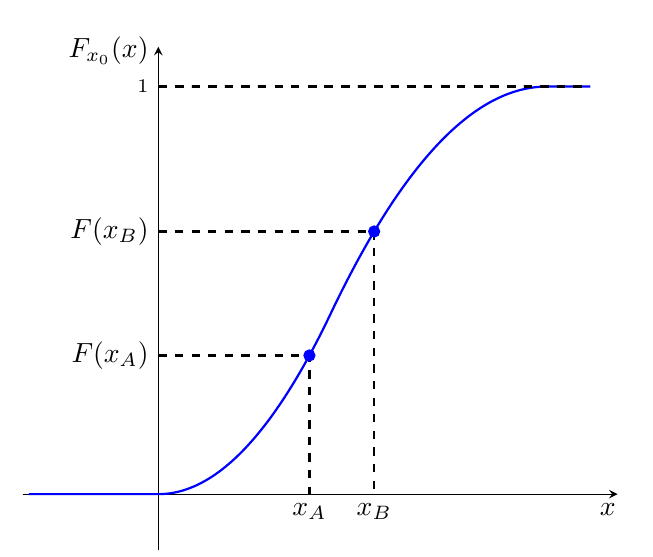
\begin{tikzpicture}[
declare function= {
    triangle(\x,\a,\b,\c) = 0+(\x<=\c)*(\x>=\a)*(pow(\x-\a,2)/((\b-\a)*(\c-\a)))+(\x<=\b)*(\x>\c)*(1-pow(\b-\x, 2)/((\b-\a)*(\b-\c)))+1*(\x>\b);
}
]
\begin{axis}[
    clip=false,
    axis lines = middle,
    axis line style={shorten >=-10pt, shorten <=-10pt},
    xlabel = {$x$}, % подпись оси x
    ylabel = {$F_{x_0}(x)$}, % подпись оси y
    xlabel style={below right},
    ylabel style={above left},	
    ymax = 1.03,
    ymin = -0.07,
    xmin = -2.5,
    xtick={0}, 
    ytick={0}
    ]
    \coordinate (a1)  at (0,{triangle(3.5, 0, 9, 4)});
    \coordinate (a2)  at (3.5,{triangle(3.5, 0, 9, 4)});
    \coordinate (a3)  at (3.5,0);
    \node at (a1) [left] {$F(x_A)$};
    \node at (a3) [below] {$x_A$};
    \draw [thick, dashed] (a1)--(a2)--(a3);
    %
    \coordinate (b1)  at (0,{triangle(5, 0, 9, 4)});
    \coordinate (b2)  at (5,{triangle(5, 0, 9, 4)});
    \coordinate (b3)  at (5,0);
    \node at (b1) [left] {$F(x_B)$};
    \node at (b3) [below] {$x_B$};
    \draw [thick, dashed] (b1)--(b2)--(b3);
    %
    \addplot[domain=-3:10, samples=300, color=blue, thick] {triangle(x, 0, 9, 4)};
    %\addplot[blue,samples=200]{triangle(x, 0, 9, 4)};
    \addplot[blue, only marks,samples at={3.5,5}]{triangle(x, 0, 9, 4)};
    \addplot[domain=0:10, samples=300, color=black, thick, dashed] {1};
    \coordinate (c1)  at (0,1);
    \node at (c1) [left] {\scriptsize $1$};
\end{axis}
\end{tikzpicture}